%\documentclass[14pt]{extarticle}
\documentclass[12pt, a4paper]{article}
\usepackage[russian]{babel}
\usepackage[utf8]{inputenc}
\usepackage[T2A]{fontenc}
\usepackage{amsfonts}
\usepackage{amsmath}
\usepackage[
left 	= 	30	mm,
right 	=	15	mm,
top 	=	20	mm,
bottom 	=	20	mm,
]{geometry}

\usepackage{indentfirst} % Красная строка

\setlength{\parindent}{1.25 cm}

\usepackage[toc,page]{appendix}

\renewcommand{\baselinestretch}{1.5}

\usepackage{titlesec}

\titleformat{\section}
{\normalfont\fontsize{14}{14}\bfseries}{\thesection}{1em}{}

\titleformat{\subsection}
{\normalfont\fontsize{14}{14}\bfseries}{\thesubsection}{1em}{}

\usepackage[intoc]{nomencl}
\renewcommand{\nomname}{Обозначения и сокращения}
\makenomenclature

%%% Математика

% Шрифты для математики
\usepackage{amsmath}
\usepackage{amsfonts}
\usepackage{amssymb}
\usepackage{cancel}
\usepackage{mathrsfs}
\usepackage{mathtools}
\usepackage{upgreek}
\usepackage{xfrac}


%%% Иллюстрации
\usepackage{graphicx}
\usepackage{subcaption}
\usepackage{wrapfig}
\usepackage[export]{adjustbox}
%\graphicspath{{./img/}}

\makeatletter % список литературы
\def\@biblabel#1{#1. }
\makeatother

% Графики
\usepackage{pgfplots}
\pgfplotsset{compat=1.3}
\usepgfplotslibrary{patchplots}
%\usepackage{patchplots}
\pgfplotsset{	width	=	14	cm,
	x label style={
		font = {\small\sffamily},
		yshift = 1mm
	},
	tick label style={
		font = {\scriptsize},
	},
	y label style={
		font = {\small\sffamily},
		yshift = -1mm,
		at={(ticklabel cs:0.5)},
		%      					rotate=90,
		anchor=near ticklabel
	},
	every tick/.style	=	{
		black, 
		line width 	= 	.5	pt
	},
	axis line style 	= 	{
		line width 	= 	.5	pt
	},
	grid style	=	{
		gray,
		dotted
	},
	minor x tick num = 1,
	minor y tick num = 1,
	no markers,
	grid = major,
	every axis/.append style	=	{
		line width	=	.7	pt
	}
}

%Подписи
\usepackage		[margin		= 10	pt,
%					font		= footnotesize, 
%labelfont	= bf, 
labelsep	= endash, 
%labelfont	= bf,
%					textfont	= sl,
margin		= 0 	pt,  
aboveskip 	= 4		pt, 
belowskip 	= -6	pt,
figurename= Рисунок] {caption}
\usepackage		[margin		= 10	pt,
font		= footnotesize, 
labelfont	= bf, 
labelsep	= endash, 
labelfont	= bf,
textfont	= sl,
margin		= 0 	pt,  
aboveskip 	= 4		pt, 
belowskip 	= 6	pt]	{subcaption}

\makeatletter
%\newcounter{figure}[section]
%\newcounter{table}[section]
\renewcommand{\thefigure}{\thesection.\@arabic\c@figure}
\renewcommand{\thetable}{\thesection.\@arabic\c@table}
\makeatother


%%% Insert pdf pages
\usepackage[final]{pdfpages}


%%% Color highlight
\usepackage{xcolor}

% Ссылки внутри текста
\usepackage{hyperref}

% Настройка листингов
\usepackage{listings}
\lstset{
	language = sql,
	extendedchars=\true,
	keepspaces=true,
	basicstyle=\scriptsize\sffamily,
	showstringspaces=\false,
	numbers=left,
	stepnumber=1,
	numbersep=5pt,
	frame=single,
	tabsize=2,
	captionpos=t,
	breaklines=true,
	breakatwhitespace=false,
	escapeinside={\#*}{*)}
}


\begin{document}
	\counterwithin{lstlisting}{section}
%	\includepdf[pages=-]{titlesheet.pdf}
	
	\setcounter{page}{3}
	
	\section*{Реферат}
Курсовой проект представляет собой реализацию Web-приложения и соответствующей базы данных, ориентированные на использование охотничьими хозяйствами. Готовое приложение предоставляет возможность производить операции над путёвками, регулировать их количество, а также получать прочую информацию, касающуюся данной области.

Приложение реализовано на языке программирования Python 3 с использованием Web-фреймворка Django. PostgreSQL был выбран в качестве СУБД.

Ключевые слова: охотничье хозяйство, заявка, путёвка, Django, PostgreSQL, Python 3, Web-приложение.

Расчётно-пояснительная записка к курсовой работе содержит 51 страницу, 34 иллюстрации, 8 таблиц и 13 источников.
	\newpage
	
	% Содержание
	\tableofcontents
	\newpage
	
%	\printnomenclature[2em]
%	В тексте писать так: $\beta$\nomenclature{$\beta$}{Вторая буква греческого алфавита}
	
	\section*{Введение}
	\addcontentsline{toc}{section}{Введение}
	
	В настоящее время процент использования информационных технологий в различных сферах растёт с каждым годом, так, согласно исследованиям \cite{Russia-in-numbers} за 2018 год он вырос на $3\%$ по сравнению с предыдущим, и такая тенденция сохраняется на протяжении нескольких лет.\\

	На сегодняшний день использование такого рода технологий позволяет любой организации без препятствий взаимодействовать с большими потоками информации. Быстрый доступ к базам данных обеспечивает оперативность обмена материалами и согласованность всей работы в целом. \\
	
	Однако внедрение подобного подхода в различные инфраструктуры происходит не равномерно, например, в Распоряжении Правительства РФ "Об утверждении Стратегии развития охотничьего хозяйства в Российской Федерации до 2030 года" \cite{doc_problems} рассматривается проблема использования консервативных и неэффективных методов работы, которые затрудняют организацию и контроль. \\
	
	Объектом разработки курсового проекта было выбрано <<Общество охотников>>, осуществляющее возможность подачи заявки и покупки путёвок. \\
	
	\textbf{Целью} работы - спроектировать и реализовать базу данных для <<Общества охотников>>, и разработать Web-приложение для взаимодействия с базой данных.\\
	Выделены следующие \textbf{задачи}:
	\begin{enumerate}
		\item[1)] провести анализ существующих решений;
		\item[2)] формализовать задание и определить необходимый функционал;
		\item[3)] осуществить обзор существующих решений;
		\item[4)] провести анализ существующих СУБД;
		\item[5)] спроектировать базу данных для хранения и структурирования данных;
		\item[6)] реализовать спроектированную базу данных с использованием выбранной СУБД;
		\item[7)] разработать соответствующее Web-приложение.
	\end{enumerate}
	  
	\newpage
	
	\section{Аналитическая часть}	
	\subsection{Обзор существующих аналогов}
	В настоящий момент существует несколько сервисов, выполняющих похожие задачи.
	
	\subsubsection{Геопортал охотничьего хозяйства России}
	Этот портал предоставляет удобный сервис для наилучшего ориентирования пользователей среди разнообразных охотничьих хозяйств. Он включает в себя набор интерактивных карт субъектов Российской Федерации с возможностью перехода по клику на информационную страницу, соответствующую выбранному элементу. \cite{maps} \\
	
	Однако набор действий на сайте очень ограничен. Так, ссылки, указывающие на возможность приобретения путёвки на охоту, перенаправляют пользователя либо на инструкцию, в которой указано, какое учреждение нужно очно посетить для оформления соответствующих документов, либо на сайт с уже устаревшей информацией. И лишь некоторые субъекты перенаправляют на сайт Госуслуг для подачи заявки онлайн. Личного кабинета у пользователя на этом портале нет. \\
	
	\subsubsection{Портал государственных и муниципальных услуг}
	Сервис поддерживает подачу заявок онлайн, для этого необходимо заполнить формы и загрузить необходимые документы. Но также обязательным условием является посещение МФЦ. Все оформленные путёвки появляются в специально отведённом разделе в личном кабинете.\\
	
	Основным неудобством в работе данных сервисов является отсутствие возможности оформления документов на охоту удалённо, в любом случае, требуется посещение специального учреждения. Также ввиду ограниченного функционала личный кабинет либо отсутствует, либо предоставляет только общую информацию, за детальным разъяснением приходится обращаться в сторонние сервисы. Поэтому в качестве одной из задач данной работы ставится выполнение указанных требований.
	
	\subsection{Формализация задачи}
	В ходе выполнения курсовой работы должно быть спроектировано и реализовано Web-приложение, предоставляющее интерфейс для работы с данными о членах организации, путёвках, прайс-листах для различных категорий пользователей (таких как, администратор, егерь, охотник). Для каждого участника должен быть определён свой набор прав и разрешённых действий.\\
	
	Кроме того, необходимо обеспечить возможность регистрации с дальнейшим подтверждением со стороны администратора. В случае положительного ответа пользователю предоставляется функционал в соответствии с его категорией.
	
	\subsection{Формализация ролей}
	Было выделено три категории пользователей.\\
	
	\textbf{Охотник} \\
		Может выполнять следующие действия.
		\begin{itemize}
			\item Просматривать:
			\begin{itemize}
				\item личную информацию;
				\item контакты всех егерей;
				\item свои одобренные путёвки и заявки на их покупку;
				\item прайс-лист по всем хозяйствам и секторам с возможностью поиска необходимого субъекта.
			\end{itemize}
			\item Отправлять:
			\begin{itemize} 
			 	\item заявки на путёвки с указанием места охоты и количества животных.
			\end{itemize}
		 	\item Отзывать:
		 	\begin{itemize}
		 		\item созданную ранее заявку.
		 	\end{itemize}
		\end{itemize}
	
		\textbf{Егерь} \\
		Ему предоставляются следующие возможности.
		\begin{itemize}
			\item Просматривать:
			\begin{itemize}
				\item личную информацию;
				\item общую информацию о всех охотниках с возможностью поиска по ФИО и номеру охотничьего билета;
				\item контакты всех егерей;
				\item прайс-лист закреплённого за ним сектора с возможностью поиска необходимого животного;
				\item заявки на охоту, а также одобренные путёвки в его сектор.
			\end{itemize}
			\item Отклонить или принять:
			\begin{itemize} 
				\item заявку на путёвку в его сектор.
			\end{itemize}
			\item Оформить:
			\begin{itemize} 
				\item новую путёвку в закреплённый за ним сектор с указанием номера билета охотника и позиции из доступного прайс-листа.
			\end{itemize}
			\item Закрыть:
			\begin{itemize}
				\item уже одобренную путёвку.
			\end{itemize}
			
		\end{itemize}
		
		\textbf{Администратор}\\
		Для него определён соответствующий набор действий.
		\begin{itemize}
			\item Просматривать:
			\begin{itemize}
				\item личную информацию;
				\item информацию о всех охотниках с возможностью поиска по ФИО и номеру билета;
				\item информацию о всех егерях с возможностью поиска по ФИО и субъекту;
				\item информацию о всех администраторах с возможностью поиска по ФИО;
				\item заявки на охоту во всех возможных хозяйствах и секторах;
				\item заявки на регистрацию в качестве охотника, егеря, администратора;
				\item выданные путёвки во всех возможных хозяйствах и секторах.
			\end{itemize}
			\item Отклонить или принять:
			\begin{itemize} 
				\item заявку на охоту в любой субъект;
				\item заявку на регистрацию в качестве охотника, егеря, администратора.
			\end{itemize}
			\item Оформить:
			\begin{itemize} 
				\item новую путёвку с указанием названия хозяйства, номера сектора, номера билета охотника и позиции из доступного прайс-листа.
			\end{itemize} 
			\item Закрыть:
			\begin{itemize}
				\item уже одобренную путёвку из любого субъекта.
			\end{itemize}
			\item Удалить аккаунт:
			\begin{itemize} 
				\item охотника;
				\item егеря;
				\item администратора (кроме себя самого).
			\end{itemize}
		\end{itemize}
	
	\subsection{Формализация данных}
	На рисунке \ref{fig1:image} приведена ER-диаграмма схемы сущностей.
	
	\begin{figure}[ph!]
		\centering
		\begin{center}
			{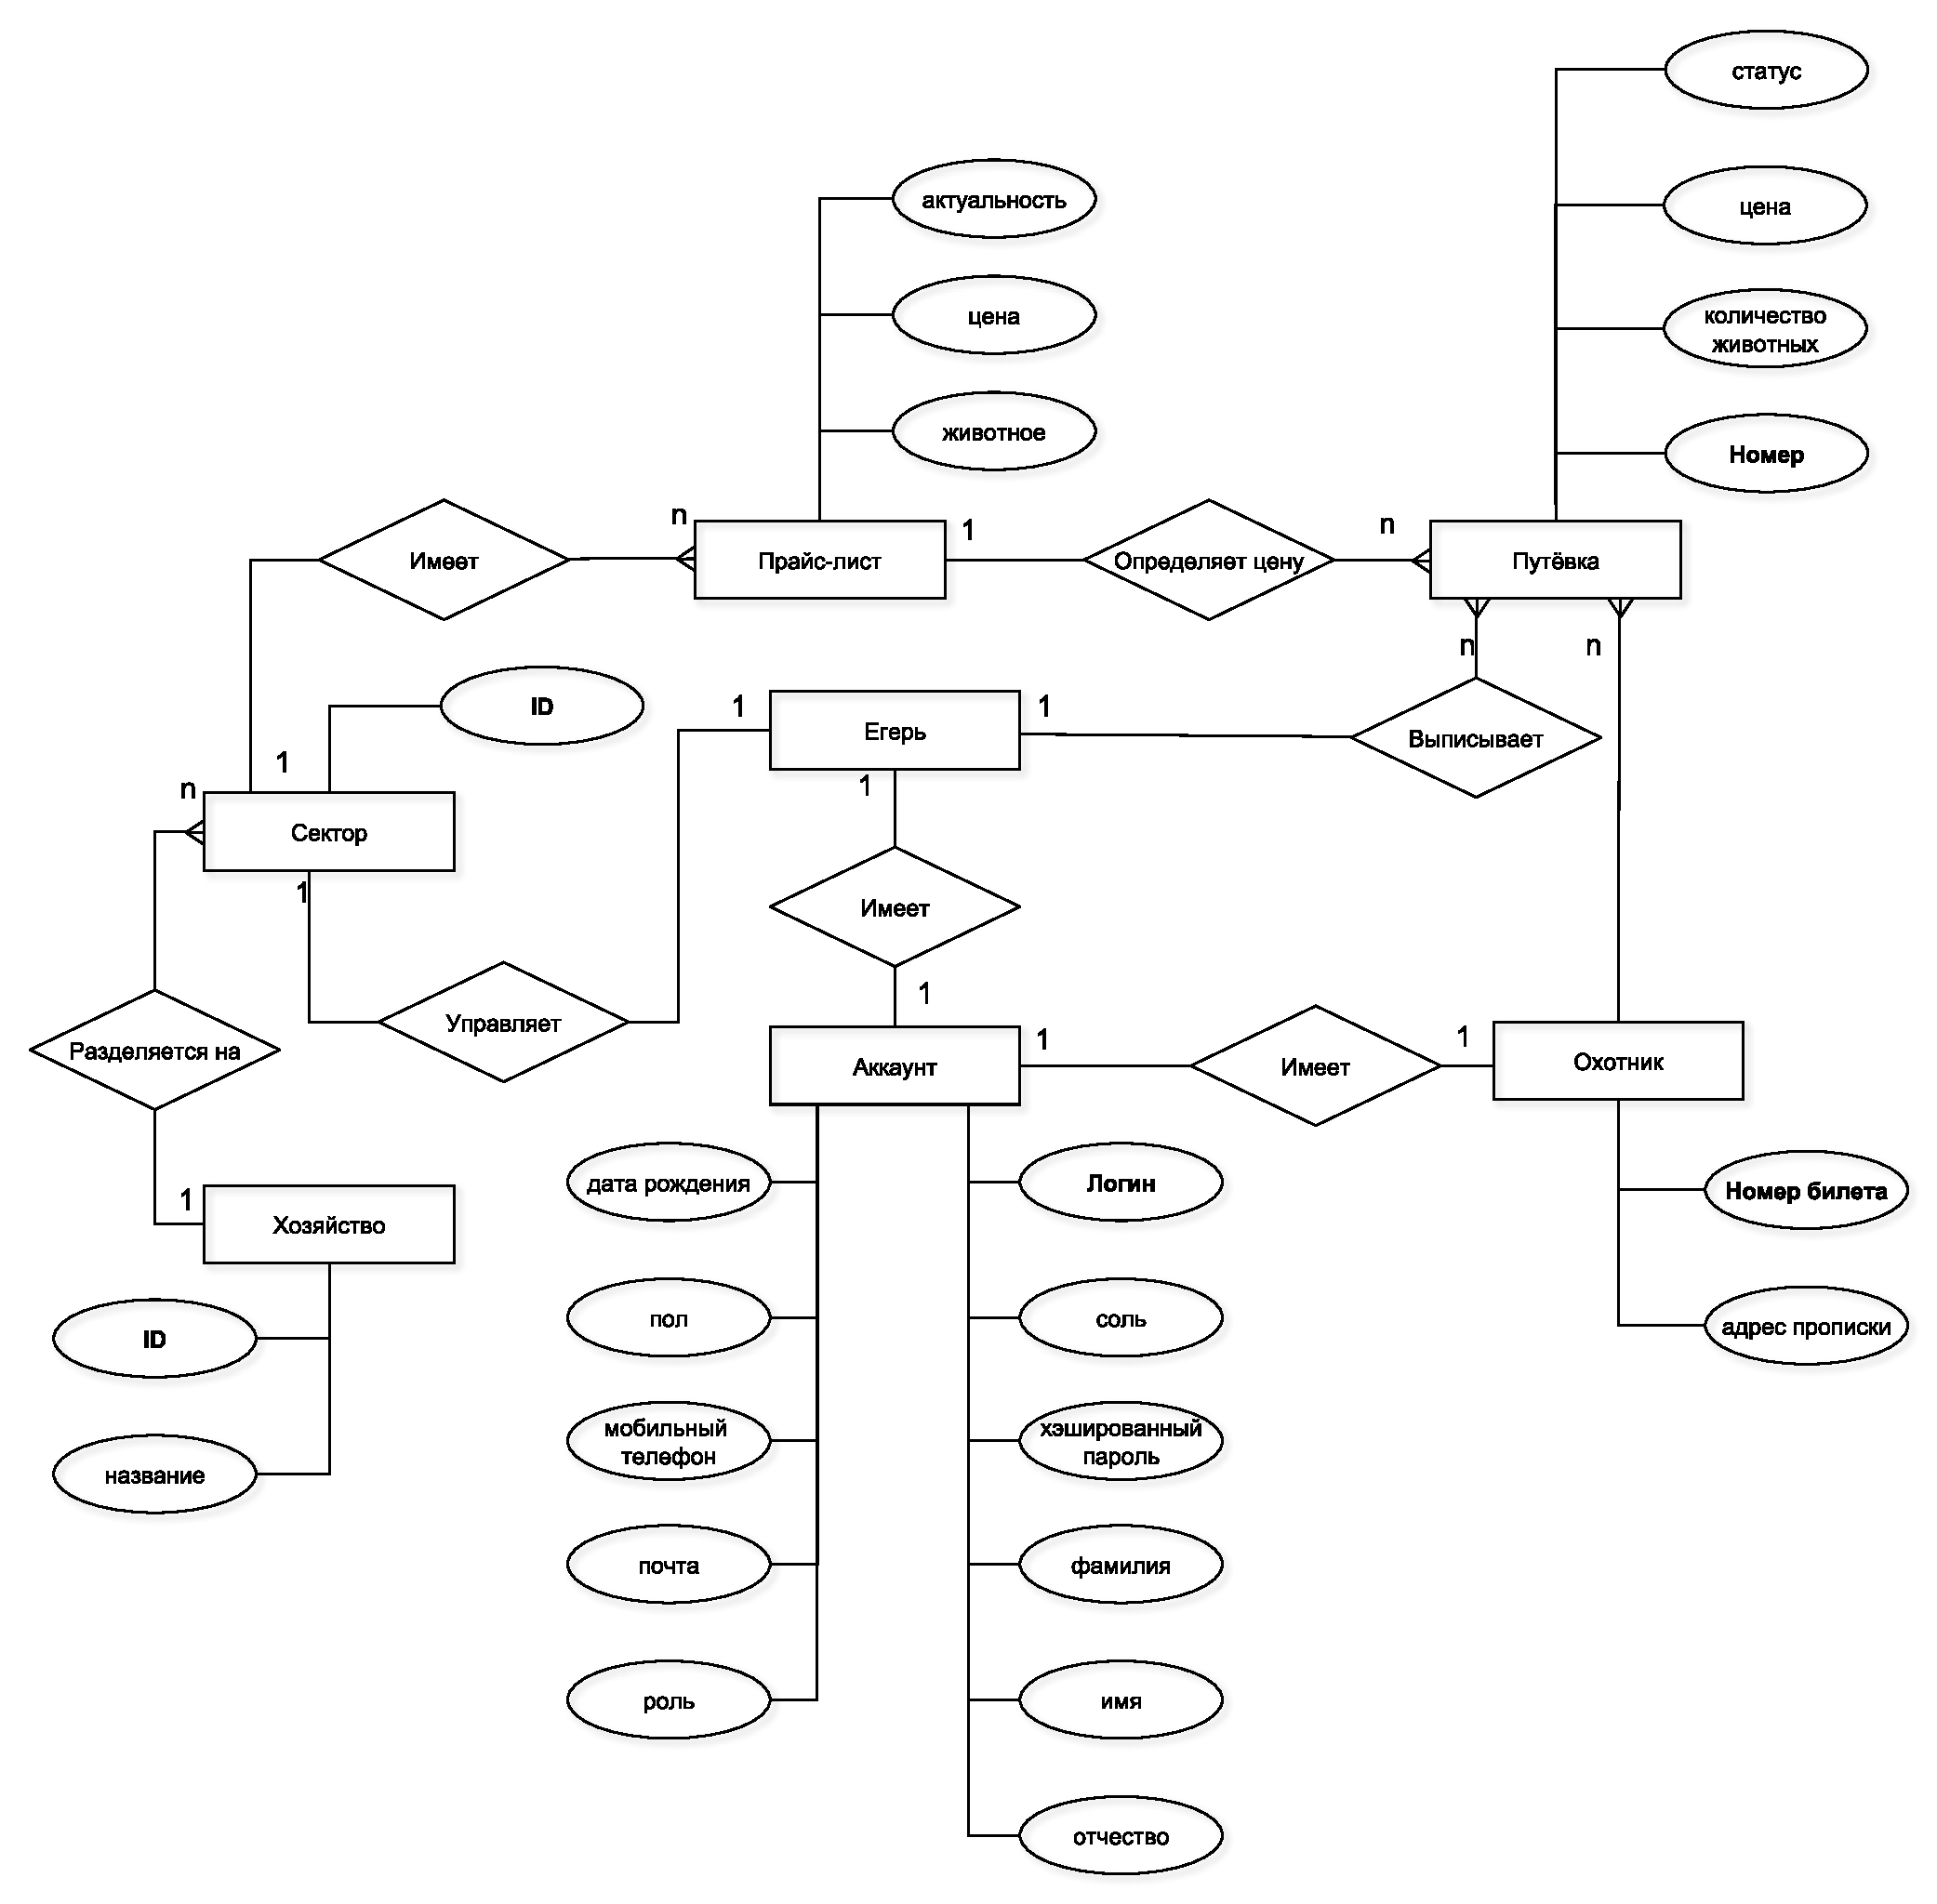
\includegraphics[scale=0.45]{schemes/er.pdf}}
			\caption{ER-диаграмма сущностей}
			\label{fig1:image}
		\end{center}
	\end{figure}

	\newpage

	\subsection{Базы данных}
	\subsubsection{Определение базы данных}
	\textbf{База данных (БД)} -  это самодокументированное собрание интегрированных записей.\\
	\textbf{Самодокументированная} - хранятся метаданные (данные о данных).\\
	\textbf{Интегрированные записи} – файлы данных.
	
	\subsubsection{Требования к БД}
	\begin{enumerate}
		\item[1)] Неизбыточность \\
		Не хранится лишняя информация.
		\item[2)] Эффективность доступа \\
		Малое время отклика на запрос.
		\item[3)] Совместное использование
		\item[4)] Безопасность
		\item[5)] Восстановление после сбоя
		\item[6)] Целостность \\
		Если есть ссылка на какой-то объект, то он должен быть. Нельзя ссылаться на несуществующие объекты.
		\item[7)] Независимость от сторонних приложений
	\end{enumerate}

	\subsubsection{Модели данных}
	\textbf{Модель данных} - это абстрактное, самодостаточное, логическое определение объектов, операторов и прочих элементов, в совокупности составляющих абстрактную машину доступа к данным, с которой взаимодействует пользователь. Эти объекты позволяют моделировать структуру данных, а операторы — поведение данных. \cite{db} \\
	
	Выделяют три основные модели данных.
	\begin{enumerate}
		\item[1)] Иерархическая \\
		Подразумевается, что элементы организованы в структуры, связанные между собой иерархическими или древовидными связями. Родитель может иметь несколько потомков. Но у потомка может быть только один предок.
		\item[2)] Сетевая \\
		У родителя также может быть несколько потомков, а у дочернего элемента — несколько предков.
		\item[3)] Реляционная \\
		Главное отличие состоит в том, что информация хранится в виде таблиц (отношений), состоящих из нескольких записей (кортежей), обладающих одним и тем же набором атрибутов, или полей. Используются чаще, чем две другие модели.
	\end{enumerate}

	Реляционная модель данных наиболее подходит для решения поставленной задачи, поскольку она более гибкая и удобная в использовании. Также она лучше всего соответствует описанным ранее отношениям между выделенными сущностями.
	
	\subsubsection{Система управления базами данных (СУБД)}
	\textbf{Система управления базами данных (СУБД)} - приложение, позволяющее создать базу данных и манипулировать данными (вставлять, обновлять, удалять и выбирать).\\
	Основные компоненты СУБД. \cite{db_systems}
	\begin{itemize}
		\item Ядро \\
		Отвечает за управление данными во внешней и оперативной памяти и журнализацию.
		\item Процессор языка БД\\
		Используется для оптимизации запросов на извлечение и изменение данных.
		\item Подсистема поддержки времени исполнения\\
		Интерпретирует программы манипуляции данными, создающие пользовательский интерфейс с СУБД.
		\item Сервисные программы\\
		Отвечают за обеспечение дополнительных возможностей.
	\end{itemize}

	\subsection*{Вывод}
	Был проведён обзор существующих решений, на основе анализа предоставляемых ими возможностей была формализована задача курсового проекта, также были определены категории пользователей и соответствующие им действия. Кроме того, приведены некоторые теоретические сведения, необходимые для дальнейшей работы.
	
	
	\newpage
	
	\section{Конструкторская часть}	
	\subsection{Use-Case диаграмма}
	На рисунках \ref{fig2:image}-\ref{fig4:image} приведены диаграммы вариантов использования для каждого актора, полная схема находится в приложении.
	
	\begin{figure}[ph!]
		\centering
		\begin{center}
			{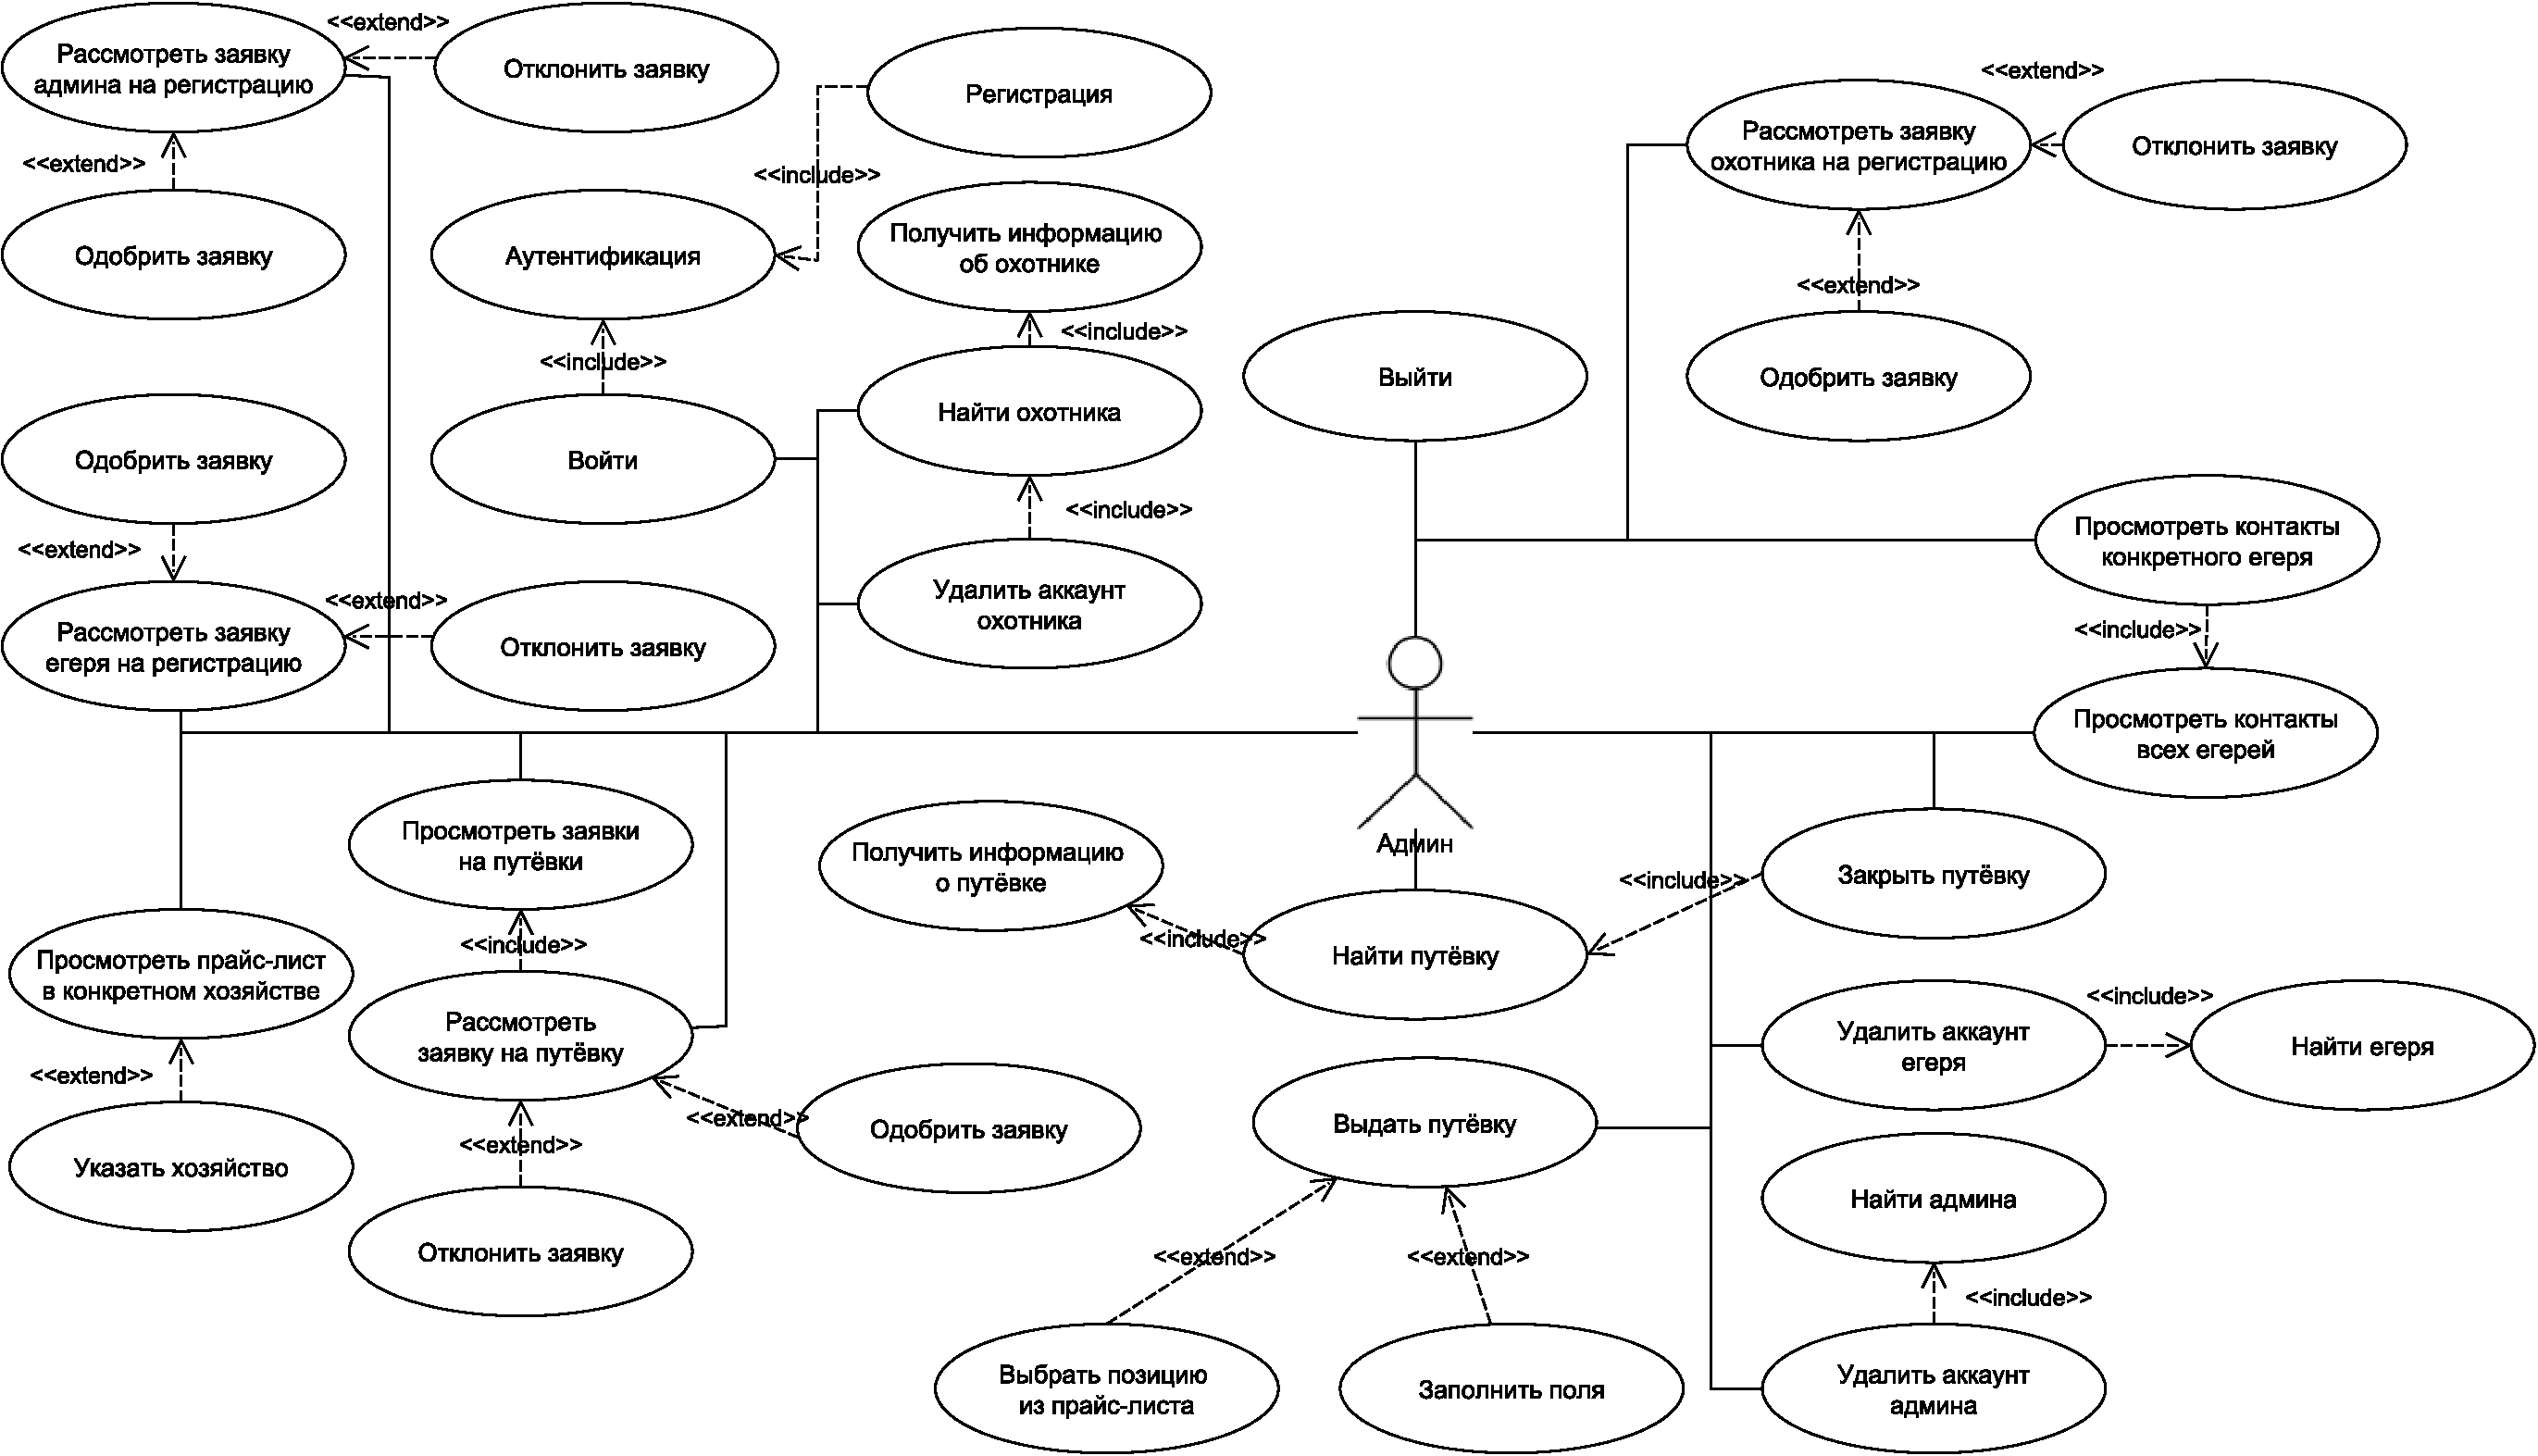
\includegraphics[scale=0.44, angle=90]{schemes/use-case_admin.pdf}}
			\caption{ER-диаграмма сущностей (администратор)}
			\label{fig2:image}
		\end{center}
	\end{figure}

	\begin{figure}[ph!]
		\centering
		\begin{center}
			{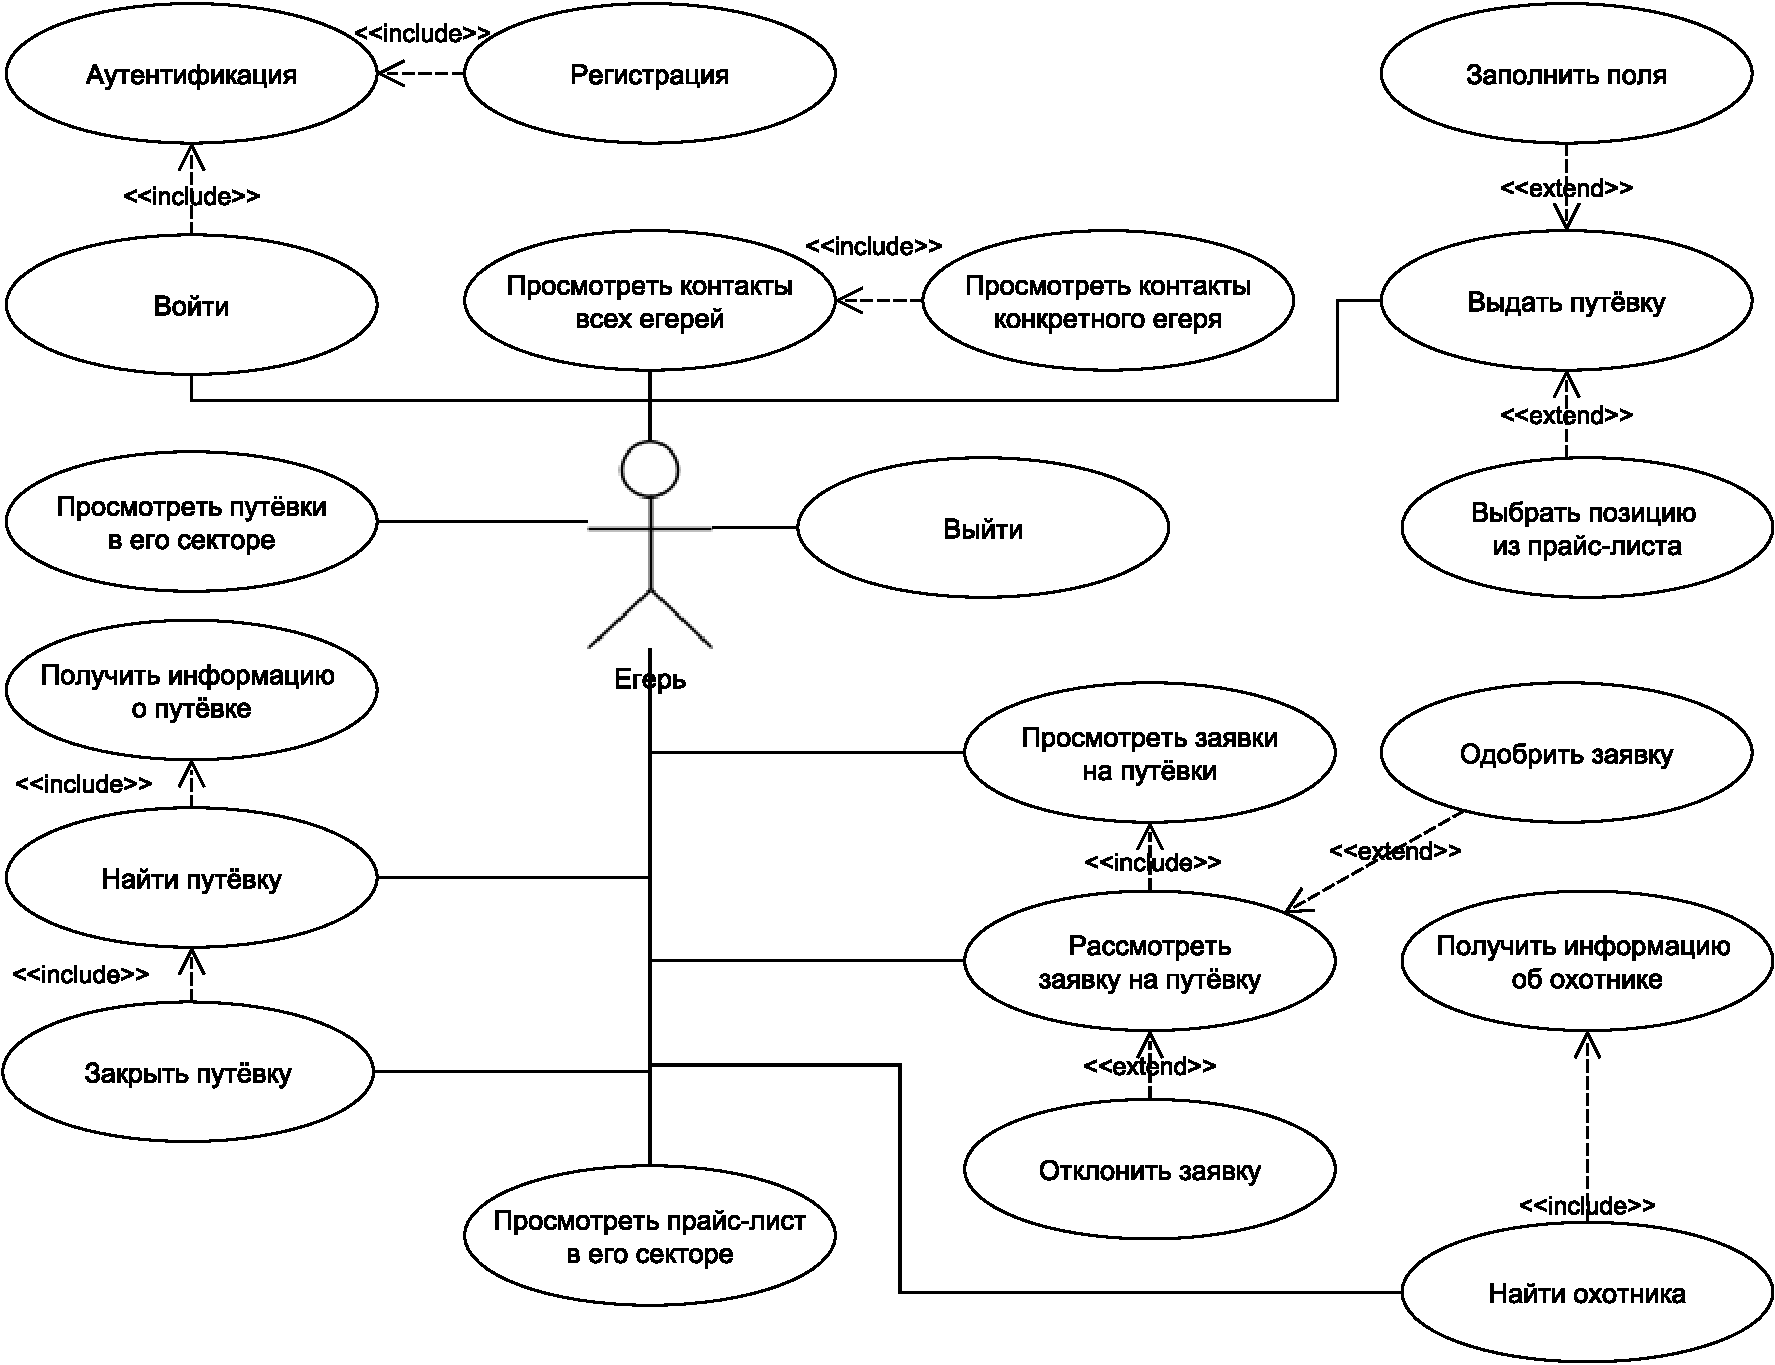
\includegraphics[scale=0.45]{schemes/use-case_huntsman.pdf}}
			\caption{ER-диаграмма сущностей (егерь)}
			\label{fig3:image}
		\end{center}
	\end{figure}

	\begin{figure}[ph!]
		\centering
		\begin{center}
			{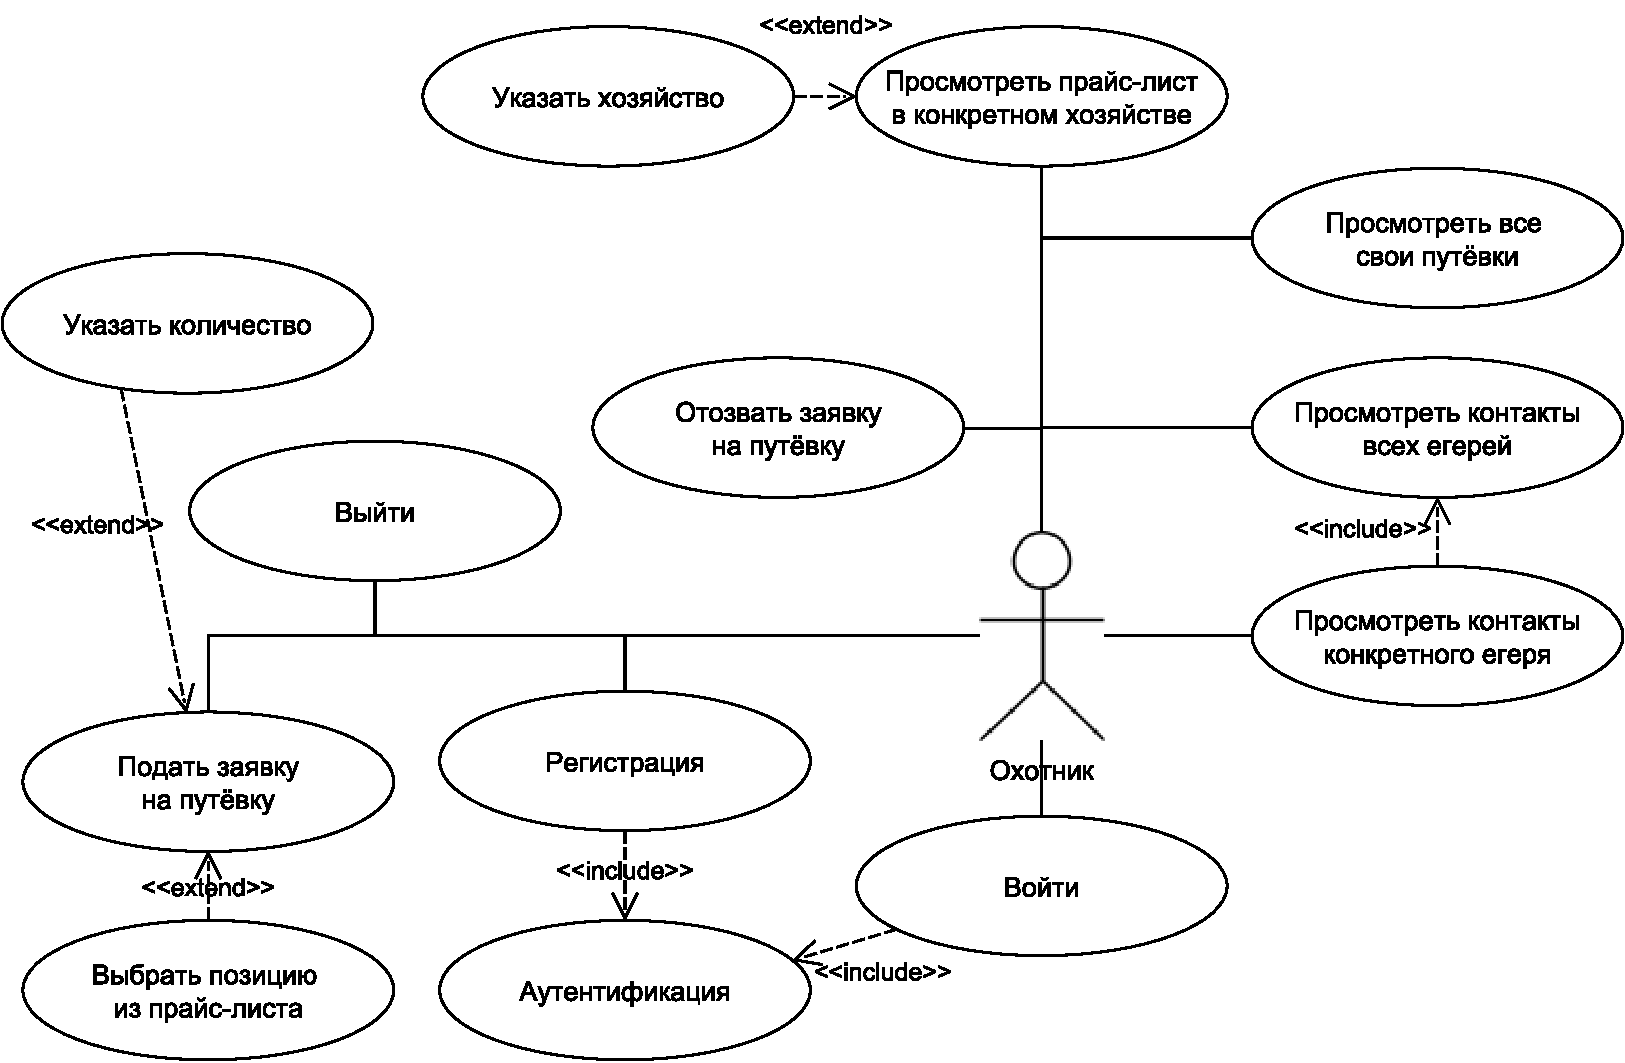
\includegraphics[scale=0.45]{schemes/use-case_hunter.pdf}}
			\caption{ER-диаграмма сущностей (охотник)}
			\label{fig4:image}
		\end{center}
	\end{figure}
	
	\newpage
	
	\subsection{ER-диаграмма сущностей БД}
	На рисунке \ref{fig5:image} приведена ER-диаграмма базы данных, на которой также указываются связи, поля таблиц и ключи.
	
	\begin{figure}[ph!]
		\centering
		\begin{center}
			{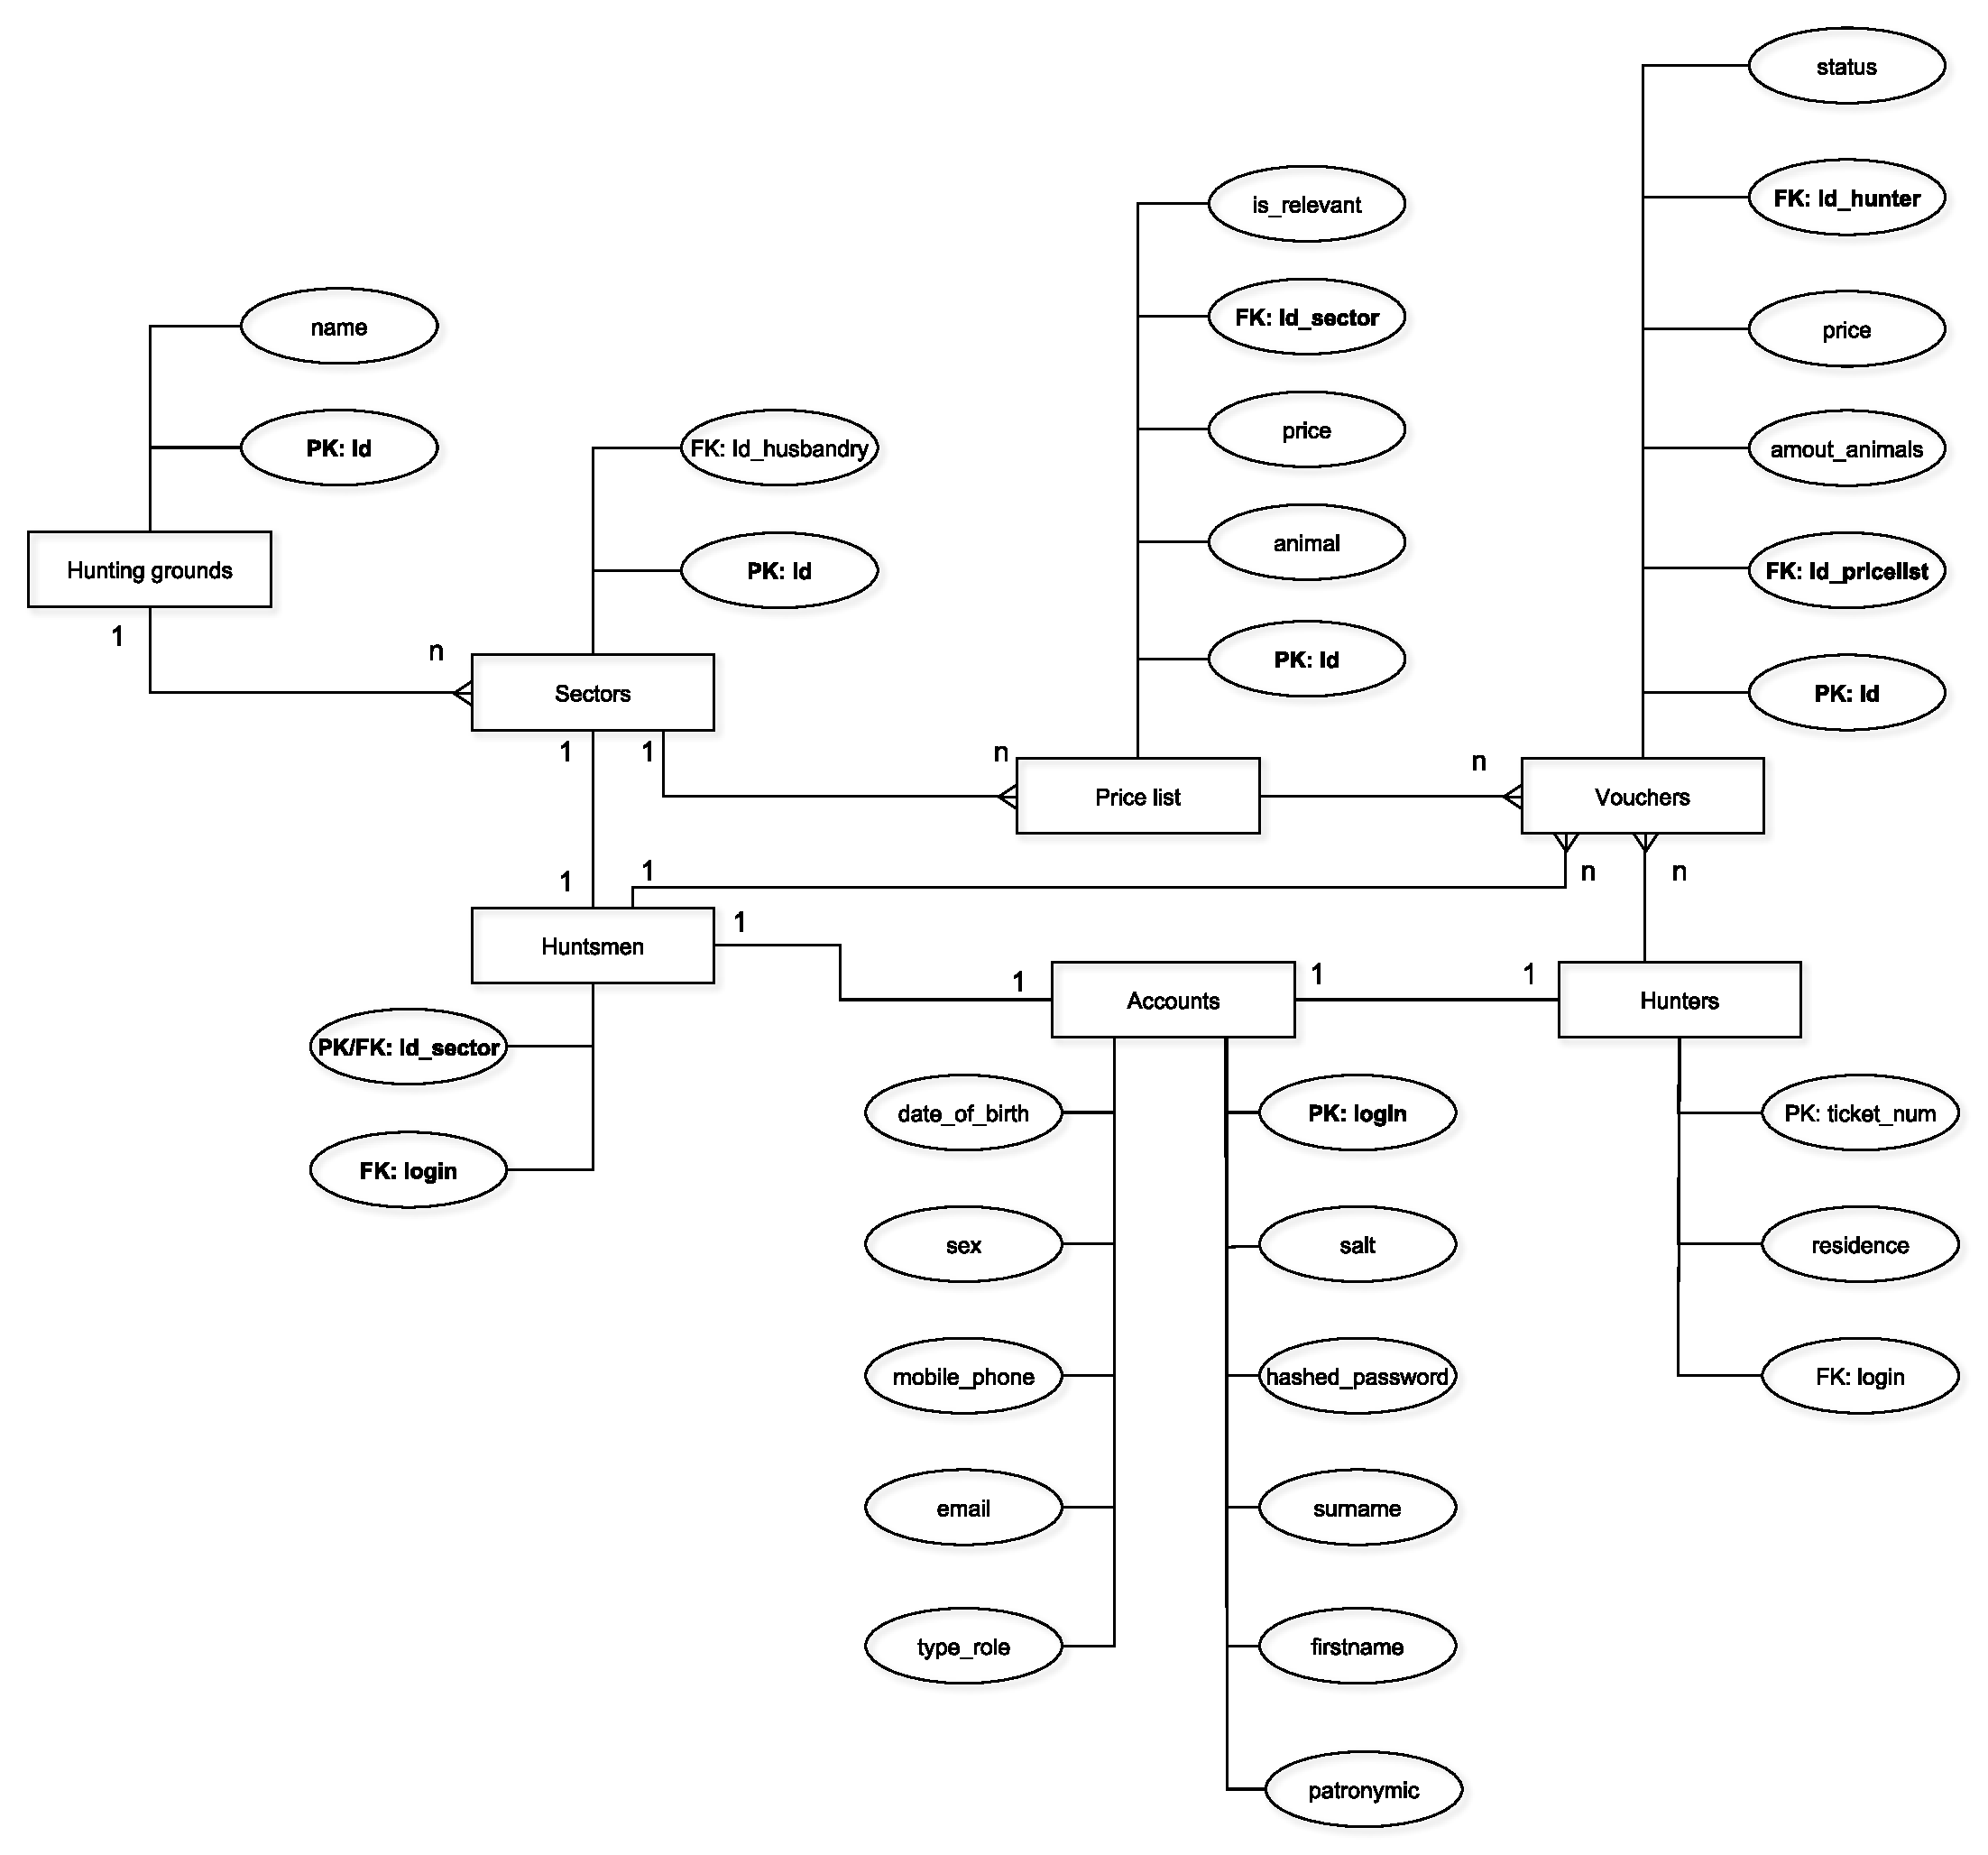
\includegraphics[scale=0.47]{schemes/ERclassic.pdf}}
			\caption{ER-диаграмма сущностей}
			\label{fig5:image}
		\end{center}
	\end{figure}

	\subsubsection{Проектирование базы данных}

	База данных должна содержать таблицы, поля и назначение которых описаны в таблицах 
	\ref{hgtable}-\ref{vouchers_table}.
	
	\begin{table}[h] 
		\begin{center}
			\caption{HuntingGrounds (таблица хозяйств)}
			\label{hgtable}
			\begin{tabular}{| p{3cm} | p{3cm} | p{8cm} |}
				\hline
				\textbf{Атрибут} 	& \textbf{Тип} & \textbf{Значение} \\
				\hline
				Id 					& Целое число &	Идентификатор, PK \\ 
				\hline
				GroundName 			& Строка &	Название \\ 
				\hline
			\end{tabular}
		\end{center}
	\end{table}

	\begin{table}[h] 
		\begin{center}
			\caption{Sectors (таблица секторов)}
			\label{sec_table}
			\begin{tabular}{| p{3cm} | p{3cm} | p{8cm} |}
				\hline
				\textbf{Атрибут} 	& \textbf{Тип} & \textbf{Значение} \\
				\hline
				Id 					& Целое число &	Идентификатор, PK \\ 
				\hline
				IdHusbandry 		& Целое число &	Идентификатор хозяйства, в состав которого входит сектор, FK \\
				\hline
			\end{tabular}
		\end{center}
	\end{table}

	\begin{table}[pt!]
		\begin{center}
			\caption{Accounts (таблица аккаунтов)}
			\label{acc_table}
			\begin{tabular}{| p{3cm} | p{3cm} | p{8cm} |}
				\hline
				\textbf{Атрибут} 	& \textbf{Тип} & \textbf{Значение} \\
				\hline
				Login 				& Строка &	Логин, PK \\ 
				\hline
				Salt 				& Строка &	Соль  \\ 
				\hline
				HashedPassword 		& Строка &	Хэшированный пароль \\ 
				\hline
				Surname 			& Строка &	Фамилия \\ 
				\hline
				Firstname 			& Строка &	Имя \\ 
				\hline
				Patronymic 			& Строка &	Отчество \\ 
				\hline
				DateOfBirth 		& Дата &	Дата рождения \\ 
				\hline
				Sex 				& Символ &	Пол \\ 
				\hline
				MobilePhone 		& Строка &	Мобильный телефон \\ 
				\hline
				Email 				& Строка &	Электронная почта \\ 
				\hline
				TypeRole 			& Строка &	Роль \\ 
				\hline
			\end{tabular}
		\end{center}
	\end{table}

	Для обеспечение безопасности используются хэширование паролей, и в базе данных в таблице \ref{acc_table} хранится только соль и хэшированный пароль.\\

	\begin{table}[pt!] 
		\begin{center}
			\caption{Huntsmen (таблица егерей)}
			\label{huntsmen_table}
			\begin{tabular}{| p{3cm} | p{3cm} | p{8cm} |}
				\hline
				\textbf{Атрибут} 	& \textbf{Тип} & \textbf{Значение} \\
				\hline
				Id 					& Целое число &	Идентификатор сектора, за которым закреплён егерь, PK, FK \\
				\hline
				Login	 			& Строка &	Логин, FK \\ 
				\hline
			\end{tabular}
		\end{center}
	\end{table}

	\begin{table}[pt!] 
		\begin{center}
			\caption{Hunters (таблица охотников)}
			\label{hunters_table}
			\begin{tabular}{| p{3cm} | p{3cm} | p{8cm} |}
				\hline
				\textbf{Атрибут} 	& \textbf{Тип} & \textbf{Значение} \\
				\hline
				TicketNum 			& Строка &	Номер охотничьего билета, PK\\
				\hline
				Residence			& Строка & 	Адрес прописки \\
				\hline
				Login	 			& Строка &	Логин, FK \\ 
				\hline
			\end{tabular}
		\end{center}
	\end{table}

	\begin{table}[pt!]
		\begin{center}
			\caption{PriceList (таблица цен на путёвки)}
			\label{price_table}
			\begin{tabular}{| p{3cm} | p{3cm} | p{8cm} |}
				\hline
				\textbf{Атрибут} 	& \textbf{Тип} & \textbf{Значение} \\
				\hline
				Id 					& Целое число &	Идентификатор, PK\\
				\hline
				Animal				& Строка & 	Название животного \\
				\hline
				Price	 			& Вещественное число &	Цена \\ 
				\hline
				IsRelevant	 		& Логический &	Флаг актуальности \\ 
				\hline
				IdSector	 		& Целое число &	Идентификатор сектора, за которым закреплена позиция, FK \\
				\hline
			\end{tabular}
		\end{center}
	\end{table}

	\begin{table}[pt!] 
		\begin{center}
			\caption{Vouchers (таблица путёвок)}
			\label{vouchers_table}
			\begin{tabular}{| p{3cm} | p{3cm} | p{8cm} |}
				\hline
				\textbf{Атрибут} 	& \textbf{Тип} & \textbf{Значение} \\
				\hline
				Id 					& Целое число &	Идентификатор, PK\\
				\hline
				AmountAnimals		& Целое число & 	Количество животных \\
				\hline
				Price	 			& Вещественное число &	Цена \\ 
				\hline
				IdHunter	 		& Строка &	Идентификатор владельца-охотника, FK \\ 
				\hline
				IdPricelist	 		& Целое число &	Идентификатор позиции из перечня цен, FK \\
				\hline
				Status				& Логический & 	Статус (ждёт решения/одобрено) \\
				\hline
			\end{tabular}
		\end{center}
	\end{table}

	\subsection{Нормальная форма модели}
	1 нф потому
	2/3
	!!!!!!!!!!!!!!!!!!!!!!!!!!!!!!!!!!!!!!!!!!!!!!!!!!!!!!!!!!!!!!!!!!!!!!!!!!!!!!!!!!!!!!!!!!!!!
	
	\subsection{Схемы триггеров}
	!!!!!!!!!!!!!!!!!!!!!!!!!!!!!!!!!!!!!!!!!!!!!!!!!!!!!!!!!!!!!!!!!!!!!!!!!!!!!!!!!!!!!!!!!!!!!

	\subsection{Архитектура приложения. Модель MVC}
	Этот шаблон проектирования предполагает разделение на три отдельных компонента: Модель (Model), Представление (View) и Контроллер (Controller). Это позволяет производить модификации какого-либо компонента независимо от других. \cite{mvc} 
	
	\textbf{Model} - компонент бизнес-логики приложения, предоставляет данные и методы работы с ними.
	
	\textbf{View} - компонент, который отвечает за взаимодействие с пользователем, необходим для отображения данных, полученных в результате работы модели.
	
	\textbf{Controller} отвечает за обработку действий пользователя, перенаправляет данные от пользователя к модели и наоборот.\\
	
	\subsection*{Вывод}
	В разделе были представлены: Use-Case диаграммы для каждой из выделенных ролей (администратора, егеря и охотника), ER-диаграмма сущностей базы данных. Также описана модель MVC, которая была выбрана для дальнейшей реализации.




	
	
	\newpage
	
	\section{Технологическая часть}
	\subsection{Средства реализации программного обеспечения}
		\subsubsection{Язык программирования}
			При разработке программного продукта был использован язык программирования Python (версия 3.7.2) \cite{python}.
			
			Данный выбор был сделан по следующим причинам.
			\begin{enumerate}
				\item[1)] Опыт работы с рассматриваемым языком.
				\item[2)] Поддержка ООП.
				\item[3)] Большое количество литературы, связанной с ЯП Python.
				\item[4)] Широкая применимость.
			\end{enumerate}
		
			В качестве среды разработки были использованы PyCharm \cite{pycharm} и Visual Studio Code \cite{vcode}, поскольку они бесплатны для студентов, удобны в процессе разработки и ранее активно использовались.

		\subsubsection{СУБД}
		Одними из наиболее популярных СУБД, используемых в настоящее время, являются Oracle, MySQL, Microsotf SQL сервер и PostgreSQL. В таблице \ref{cmptable} приведено их сравнение.
		
		\begin{table}[pt!] 
			\begin{center}
				\caption{Сравнение СУБД}
				\label{cmptable}
				\begin{tabular}{| c | l | l |}
					\hline
					\textbf{СУБД} 	& \textbf{Преимущества} & \textbf{Недостатки} \\
					\hline
					Oracle 			&  & - Платное использование \\ 
									& - Широкий функционал & - Необходимость в дополнительных \\
									& - Ориентирован на работу с большими &  ресурсах \\
									& БД & \\
					\hline
					MySQL 			& - Есть бесплатная версия &	- Есть платные версии для \\
									&  & коммерческого использования \\ 
									& - Исчерпывающая документация & - Для бесплатной версии доступна \\
									& - Простой интерфейс & только платная поддержка \\
									& - Хорошо справляется с большими & - Отсутствует встроенная поддержка \\
									& объёмами данных & XML \\
					\hline
					Microsotf SQL  	& - Низкий порог вхождения &	- Высокая цена для юридических \\
					сервер 			& - Стабильность в работе & лиц \\ 
									& - Возможность регулировать и  & - Требуется много дополнительных \\
									& отслеживать уровень & ресурсов \\ 
									& производительности &  \\
					\hline
					PostgreSQL 		& - Бесплатная & - Низкая скорость выполнения \\ 
									& - Подробная документация & пакетных операций\\
									& - Поддержка json & - Поддерживается не всеми \\
									&& библиотеками \\
					\hline
				\end{tabular}
			\end{center}
		\end{table}
	\newpage
	
	Поскольку есть опыт работы с такой СУБД, как PostgreSQL \cite{postgresql}, то это средство было выбрано для реализации текущей задачи.
	
	Что касается ORM (Object-relational mapping), то был выбран peewee \cite{peewee}, поскольку также хорошо знаком, так как активно использовался ранее.
	
	\subsubsection{Web-фреймворк}
	Django \cite{django} был выбран в качестве Web-фреймворка по следующим причинам.
	\begin{itemize}
		\item Использует шаблон проектирования MVC, который был выбран ранее.
		\item Работает с большим количеством дополнительных функций, которые значительно упрощают работу с аутентификацией пользователя, картами сайта и т.д.
		\item Масштабируемость.
	\end{itemize}

	\subsection{UML-диаграммы}
		\subsubsection{Компонент доступа к данным}
		Доступ к данным реализован с помощью паттерна проектирования Repository. Соответствующая UML-диаграмма представлена на рисунке \ref{fig6:image}.
		
		\begin{figure}[ph!]
			\centering
			\begin{center}
				{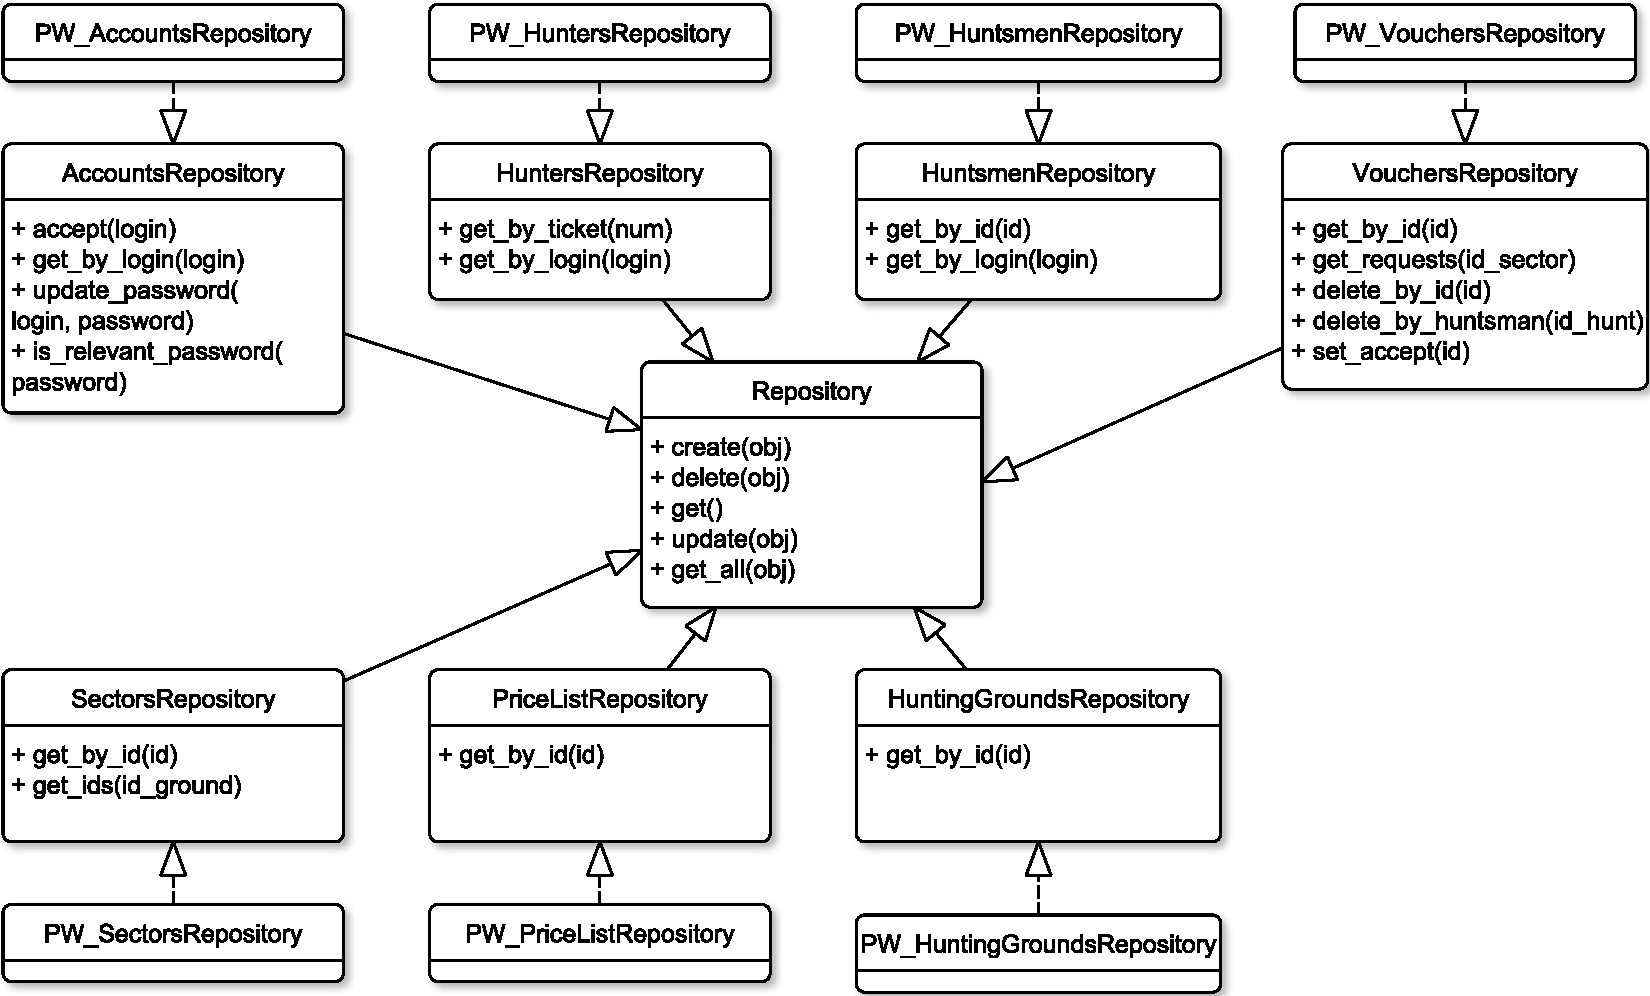
\includegraphics[scale=0.6]{schemes/uml_access_rep.pdf}}
				\caption{UML-диаграмма компонента доступа к данным}
				\label{fig6:image}
			\end{center}
		\end{figure}
		\newpage
	
		\subsubsection{Компонент бизнес-логики}
		Этот компонент выполняет основную обработку данных, соответствующая UML-диаграмма представлена на рисунке \ref{fig7:image}.
		
		\begin{figure}[ph!]
			\centering
			\begin{center}
				{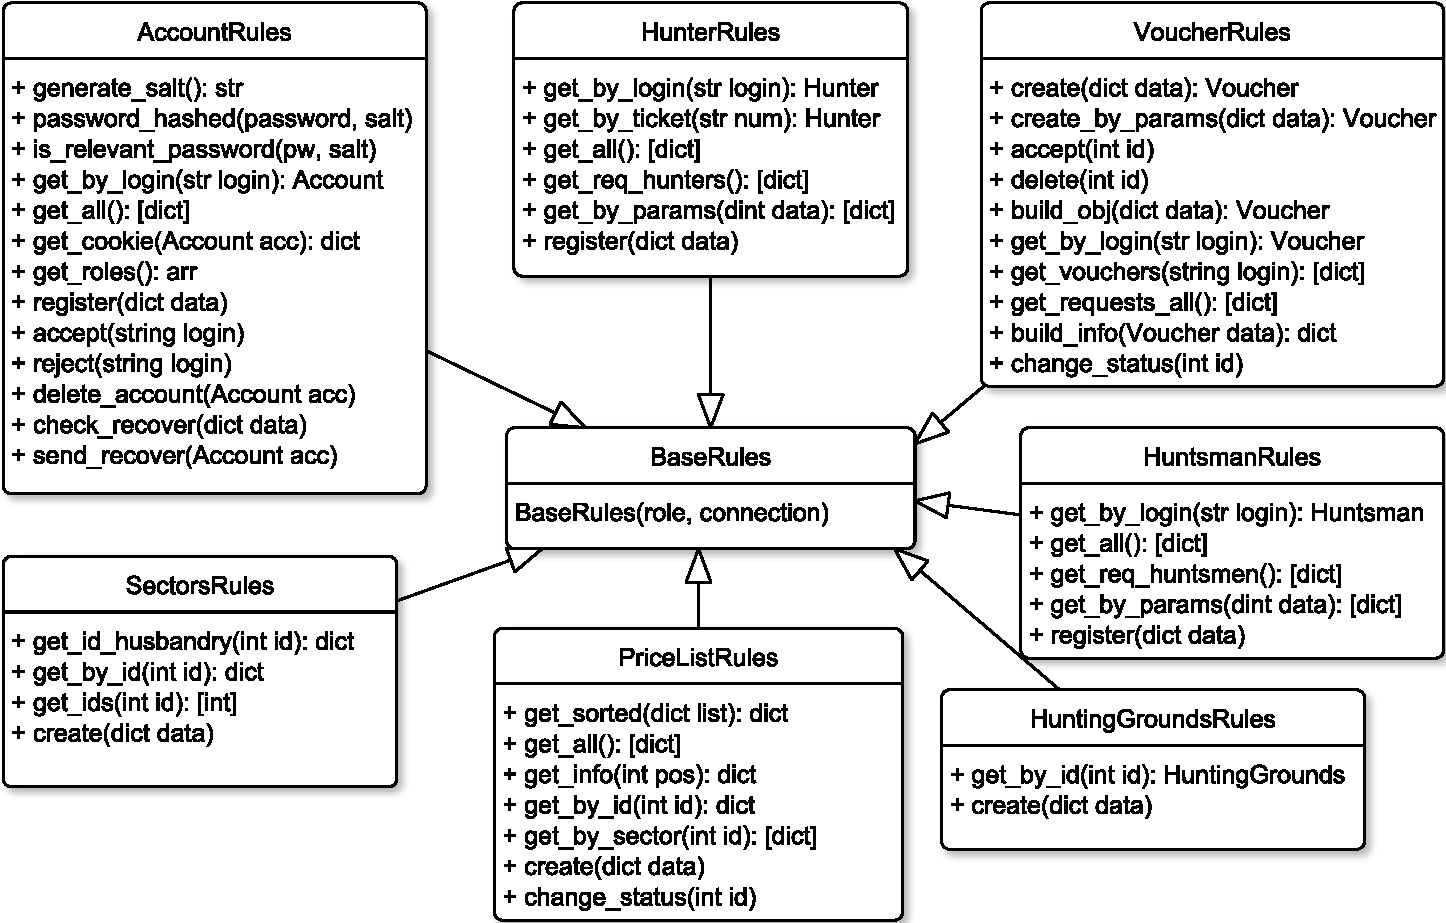
\includegraphics[scale=0.6]{schemes/uml_business.pdf}}
				\caption{UML-диаграмма компонента бизнес-логики}
				\label{fig7:image}
			\end{center}
		\end{figure}
	
		\subsubsection{Компонент представления}
		UML-диаграмма компонента, отвечающего за отображение web-страниц, изображена на рисунке \ref{fig8:image}.
		
		\begin{figure}[pt!]
			\centering
			\begin{center}
				{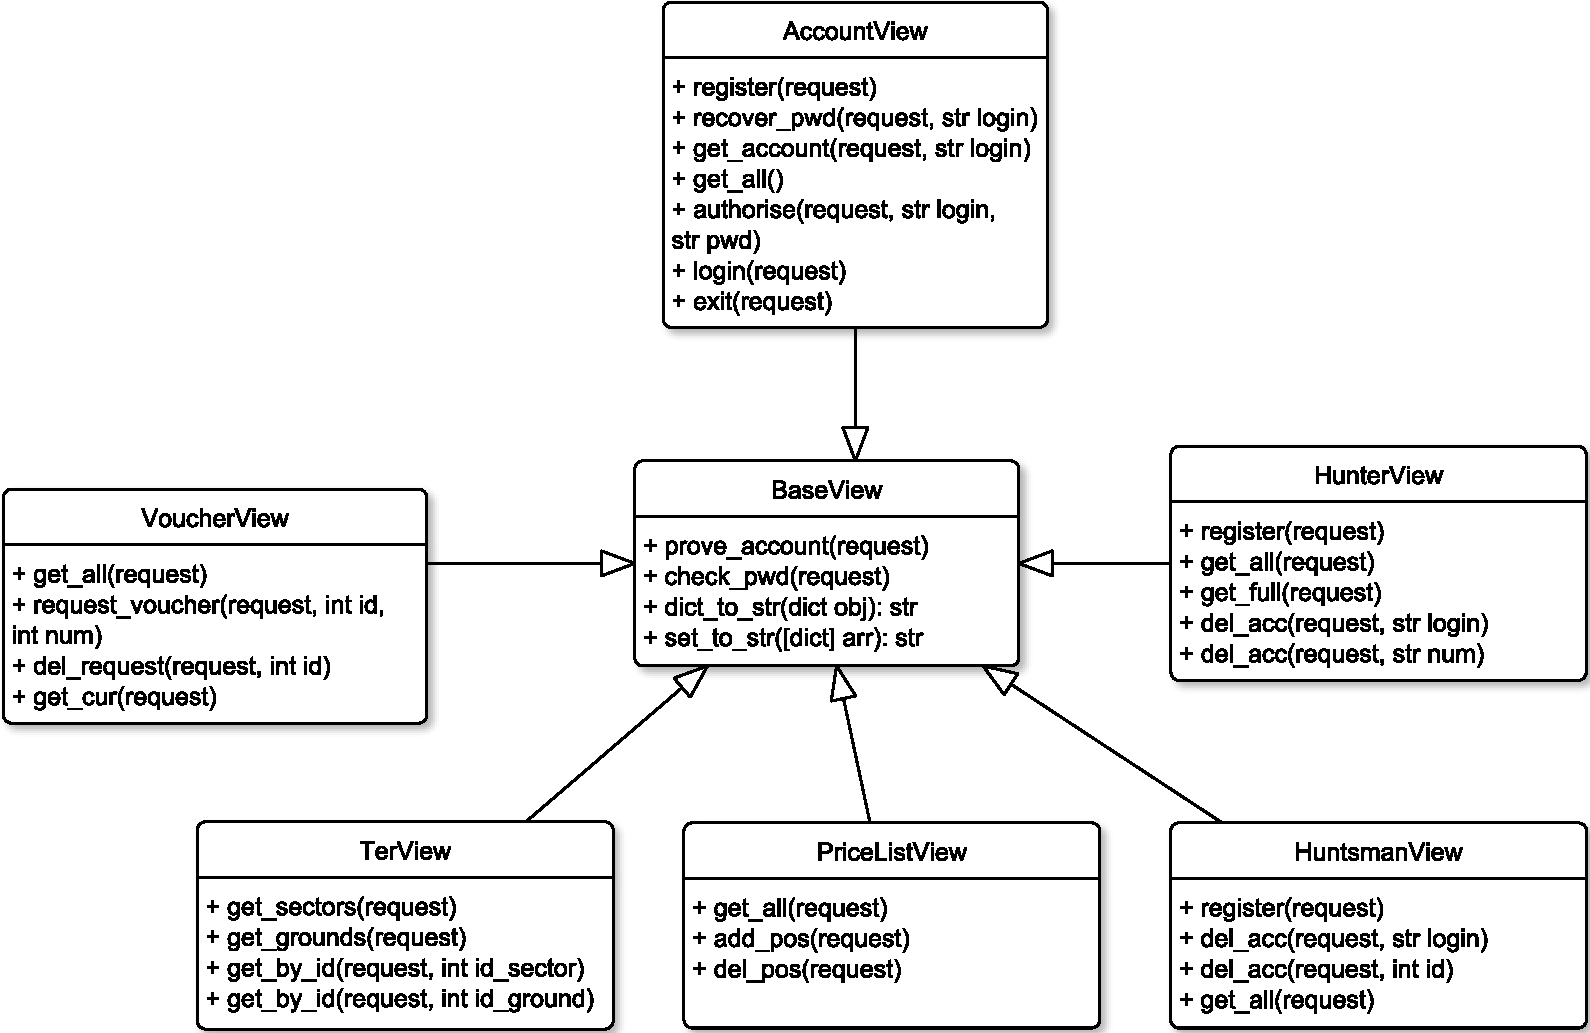
\includegraphics[scale=0.6]{schemes/webGUI.pdf}}
				\caption{UML-диаграмма компонента бизнес-логики}
				\label{fig8:image}
			\end{center}
		\end{figure}
		\newpage
	
		\subsubsection{Диаграмма приложения}
		Все приведённые выше UML-диаграммы \ref{fig6:image}-\ref{fig8:image} можно объединить в одну - диаграмму-приложения, которая находится на рисунке \ref{fig9:image}.
		
		\begin{figure}[ph!]
			\centering
			\begin{center}
				{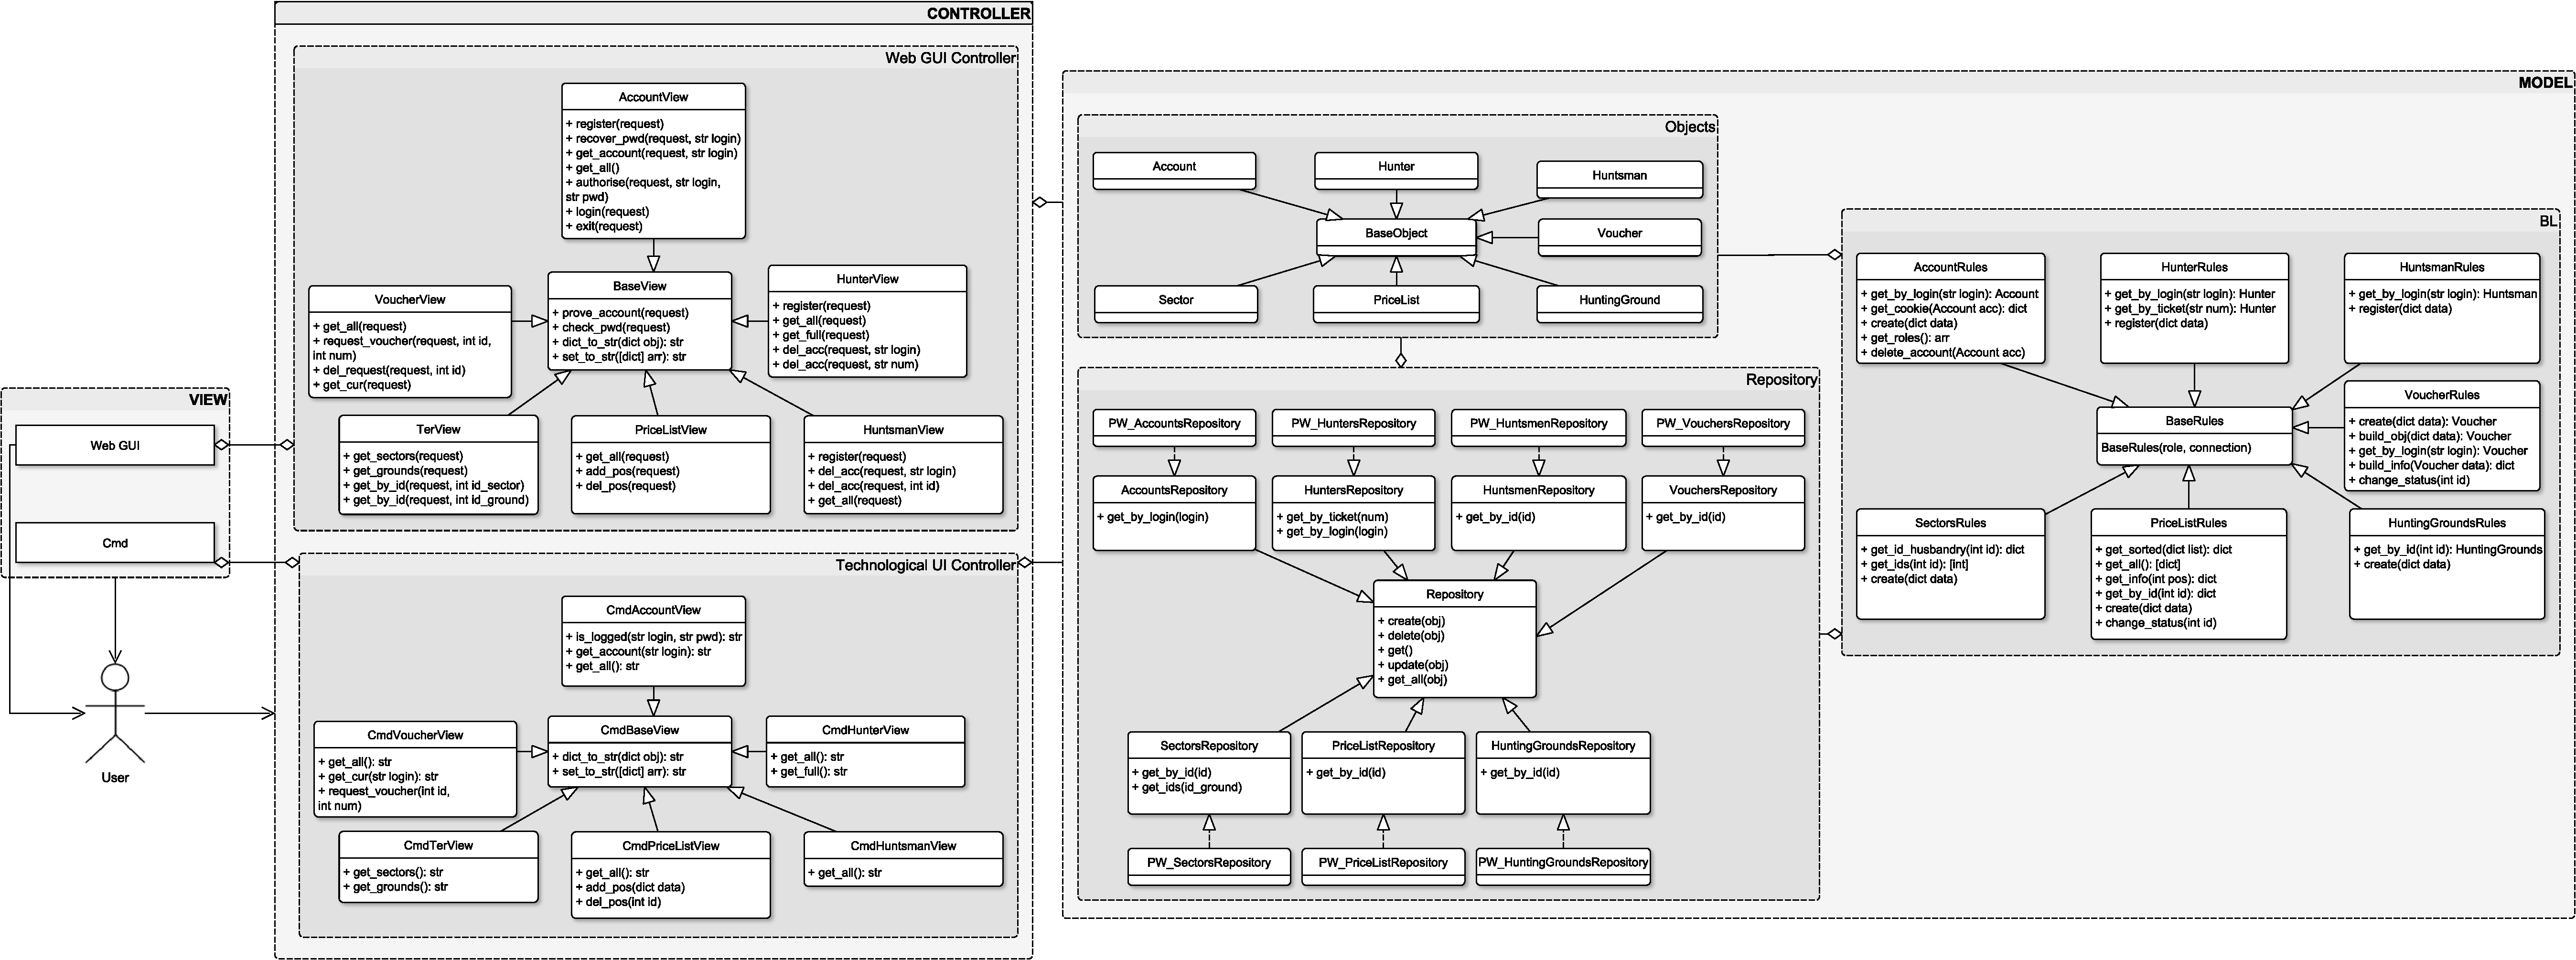
\includegraphics[scale=0.28, angle=90]{schemes/uml_full.pdf}}
				\caption{UML-диаграмма компонента бизнес-логики}
				\label{fig9:image}
			\end{center}
		\end{figure}
	\newpage
	
	\subsection{Реализация базы данных}
	!!!!!!!!!!!!!!!!!!!!!!!!!!!!!!!!!!!!!!!!!!!!!!!!!!!!!!!!!!!!!!!!!!!!!!!!!!!!!!!!!!!!!!!!!11
	\subsubsection{Создание таблиц}
	\subsubsection{Наполнение таблиц}
	\subsubsection{Реализация триггеров}
	\subsubsection{}
	
	\subsection{Интерфейс приложения}
	Для визуальной демонстрации приложения рассмотрим страницы, которые задействуются при оформлении путёвки. Сделать это может как охотник, так и егерь с администратором. 
	Для того, чтобы подать заявку на путёвку пользователь должен из верхнего меню (рисунок \ref{fig10:image}) навести мышкой на пункт <<ПУТЁВКИ>>, и затем, из выпадающего списка выбрать действие <<Купить>>.
	
	\begin{figure}[h]
		\centering
		\begin{center}
			{\includegraphics[scale=0.34]{schemes/screens/start.png}}
			\caption{Переход на страницу подачи заявки на путёвку}
			\label{fig10:image}
		\end{center}
	\end{figure}

	После этого охотник попадает на страницу, изображенную на рисунке \ref{fig11:image}. На ней приведён полный список всех доступных путёвок по всем хозяйствам и секторам. Используя мышь или правую полосу прокрутки можно ознакомиться со всем списком. 
	
	Каждая позиция из списка содержит информацию о месте (название хозяйства) и номере сектора, названии животного, на которого выдаётся разрешение, и цена за 1 единицу. 
	
	В поле <<Количество>> пользователь может указать, на сколько животных он хотел бы оформить путёвку. Для этого достаточно нажать кнопкой мыши на это поле в соответствующей строке из прайс-листа. Пользователь может указать число от 1 до 99, причём чтобы контролировать число отстреленных животных только егерь, закрепленный за данным сектором, или администратор может принимать решение одабривать такую заявку или, наоборот, отклонить. 
	
	\begin{figure}[h]
		\centering
		\begin{center}
			{\includegraphics[scale=0.34]{schemes/screens/menu.png}}
			\caption{Прайс-лист доступных путёвок}
			\label{fig11:image}
		\end{center}
	\end{figure}

	Если охотник введёт некорректные данные (например, как на рисунке \ref{fig12:image}) и попробует оформить заявку, нажав на <<Отправить заявку>>
	
	\begin{figure}[h]
		\centering
		\begin{center}
			{\includegraphics[scale=0.34]{schemes/screens/wrong_num.png}}
			\caption{Некорректный ввод данный в поле <<Количество>>}
			\label{fig12:image}
		\end{center}
	\end{figure}
	
		
		 
		
	
	\newpage
	
	\newpage
	\begin{thebibliography}{9} 
		\addcontentsline{toc}{section}{Литература}
		
		\bibitem{Russia-in-numbers} \textbf{Россия} в цифрах. 2020: Крат.стат.сб./Россат- М., 2020 - 550 с. ISBN 978-5-89476-488-7.
		
		\bibitem{doc_problems} Распоряжение Правительства Российской Федерации от 03.07.2014 N 1216-р <Об утверждении Стратегии развития охотничьего хозяйства в Российской Федерации до 2030 года> // СПС <<Консультант Плюс>> 2021 
		
		\bibitem{maps} Геопортал охотничьего хозяйства России [Электронный ресурс]. Режим доступа: https://huntmap.ru/ (дата обращения 23.03.2021).
		
		\bibitem{db} Дейт К. Дж. Введение в системы баз данных. — 8-е изд. — М.: «Вильямс», 2006. — 1328 с. — ISBN 0-321-19784-4.
		
		\bibitem{db_systems} Коннолли Т., Бегг К. Базы данных. Проектирование, реализация и сопровождение. Теория и практика — 3-е изд. — М.: Вильямс, 2003. — 1436 с. — ISBN 0-201-70857-4.
		
		\bibitem{mvc} Джесс Чедвик и др. ASP.NET MVC 4: разработка реальных веб-приложений с помощью ASP.NET MVC — М.: «Вильямс», 2013. — 432 с. — ISBN 978-5-8459-1841-3.
		
	\end{thebibliography}
	\newpage
	
%	\input{section/introduction.tex}
%	\section{Раздел первый}
%	Немного текста Немного текста Немного текста Немного текста Немного текста Немного текста Немного текста Немного 
	
%	\subsection{ghbdtn}
	
%	текста Немного текста Немного текста Немного текста Немного текста Немного текста Немного текста Немного текста 
	
%	\begin{figure}
%		\caption{Подпись}
%	\end{figure}
	
%	Немного текста Немного текста Немного текста Немного текста Немного текста Немного текста Немного текста Немного текста Немного текста Немного текста Немного текста 
%	\input{section/filename.tex}
%	...
%	\section{}
%	\input{section/filename.tex}
%	\section*{Заключение}
%	\addcontentsline{toc}{section}{Заключение}
%	\input{section/conclusion.tex}
	
%	\begin{thebibliography}{9} 
%		\addcontentsline{toc}{section}{Литература}
%		\bibitem{lamport94} Leslie Lamport, \emph{\LaTeX: a document preparation system}. Addison Wesley, Massachusetts, 2nd edition, 1994. 
%	\end{thebibliography}
	
%	\section*{Приложения}
%	\addcontentsline{toc}{section}{Приложения}
%	\subsection*{Приложение 1}
%	\addcontentsline{toc}{subsection}{Приложение 1}
%	\input{appendix/appendix_1.tex}
\end{document}
